\chapter{Arhitektura i dizajn sustava}
		
		Arhitektura se može podijeliti na nekoliko podsustava:
		 \begin{itemize}
			\item Poslužitelj frontenda
			\item Frontend (prvi dio web aplikacije)
			\item Poslužitelj backenda
			\item Backend (drugi dio web aplikacije)
			\item Baza podataka 
		\end{itemize}
		
		\begin{figure}[H]
			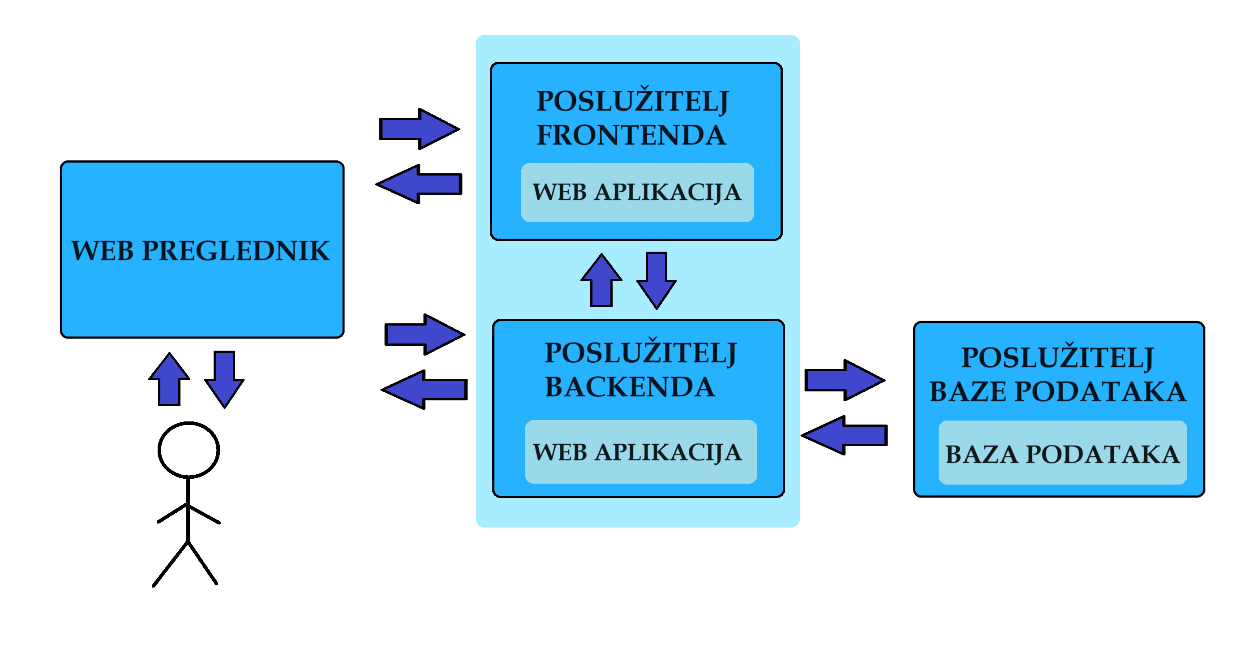
\includegraphics[width=\textwidth]{slike/arhitekturaSustava.PNG} %veličina u odnosu na širinu linije
			\caption{Arhitektura sustava}
			\label{fig:promjene9} %label mora biti drugaciji za svaku sliku
		\end{figure}
		
		 \underbar{\textit{Web preglednik}} je program koji omogućuje korisnicima pregled web sadržaja, a to uključuje web stranice i njihov raznolik sadržaj (slike, dijagrami...). Web preglednik je i okolina u kojoj se mogu izvršiti skripte (potrebno npr. kod client-side renderinga). Jedna od glavnih funkcionalnosti web preglednika je slanje zahtjeva prema web poslužiteljima.
		 	
		 \underbar{\textit{Frontend poslužitelj}} je poslužitelj koji komunicira s web preglednikom klijenta preko HTTP (\textit{engl. Hyper Text Transfer Protocol}) protokola. Na frontend poslužitelju se nalazi frontend dio web aplikacije čije dijelove frontend poslužitelj vraća klijentu na zahtjev (npr. pri početnom otvaranju stranice).
		 
		 \underbar{\textit{Backend poslužitelj}} je poslužitelj na kojem se nalazi backend dio aplikacije. Backend poslužitelj omogućuje slanje i primanje zahtjeva backend dijelu aplikacije. Backend poslužitelj preko HTTP protokola komunicira s frontendom ili web preglednikom klijenta. Ovaj poslužitelj komunicira i s poslužiteljem baze podataka preko TCP (eng. Transmission Control Protocol) protokola.
		 
		 \underbar{\textit{Web aplikacija}} dijeli se na frontend i backend. Zadaća frontend dijela je oblikovanje prikaza podataka, a potrebne podatke može zatražiti od backenda. Zadaća backend dijela je dohvaćanje podataka iz baze te njihova obrada i prosljeđivanje frontendu u određenom obliku. Komunikacija između frontenda, backenda, baze i web preglednika odvija se preko zahtjeva.
		 
		 \underbar{\textit{Baza podataka}} sadrži sve informacije o korisničkim računima, korisnicima te porukama koje korisnici šalju unutar web aplikacije.\\
		 	
		 Razvojni okvir koji smo odabrali za razvijanje backend dijela aplikacije jest Spring (programski jezik Java). Za razvoj frontend dijela aplikacije odlučili smo se za razvojni okvir React (programski jezik JavaScript). Odabrano razvojno okruženje je IntelliJ IDEA. Baza podataka napravljena je koristeći PostgreSQL.\\
		 
		 Za razvoj backenda se koristio razvojni okvir Spring MVC (Model - Pogled - Nadglednik) koji je dio Springa. Backend je po tome organiziran u 3 sloja koja međusobno komuniciraju:
		 \begin{itemize}
		 	\item Controller
		 	\item Service
		 	\item Repository
		 \end{itemize} 
		 \underbar{Controller} predstavlja vanjsko sučelje web aplikacije. Ovaj sloj prihvaća nadolazeće HTTP zahtjeve, poziva potrebne usluge koristeći razrede Service te vraća odgovor klijentu. \\
		 \underbar{Service} ostvaruje funkcionalnosti koje nudi aplikacija, predstavlja logiku programa. Ostvaruje usluge, a pritom može koristiti i druge Service razrede te može zatražiti podatke od sloja Repository.\\
		 \underbar{Repository} omogućuje komunikaciju s bazom podataka te izvlačenje podataka iz nje. Korišteno je sučelje JpaRepository koje omogućuje da se s bazom komunicira bez SQL upita - umjesto njih se koriste i modeli domene podataka. To su razredi koji predstavljaju strukturu tablica baze (entities).\\
		 Prilikom korištenja Spring MVC-a, klijentska strana predstavlja pogled, Controller sloj predstavlja nadglednika, a model je ostvaren slojevima Service i Repository. \\
		 
		 
		 Arhitektura web aplikacije temelji se na single-page application principu kojeg omogućuje razvojni okvir React. Pri početnom otvaranju web aplikacije, web preglednik korisnika uputi zahtjev frontend serveru koji mu vraća sve odgovarajuće datoteke potrebne za prikaz stranice u pregledniku (koristi se princip client-side rendering). Ovisno o prosljeđenim podacima, web preglednik prilikom obrađivanja ulaznih podataka korisnika (klik na pojedini gumb, otvaranje nove stranice) šalje zahtjeve backend serveru (ako su potrebni određeni podaci za prikaz React komponente) ili frontend serveru (za dohvat datoteka potrebnih za prikaz novog dijela stranice).
		 
		 
		  

	
		

		

				
		\section{Baza podataka}
			
		
		Za našu web aplikaciju koristiti ćemo relacijsku bazu podataka koja je industrijski standard te najjednostavniji način za rješenje našeg problema. Osnovni element baze je relacija čija su obilježja njeno ime i atributi. Glavna zadaća naše baze je spajanje njenih korisnika i sustava s korisnikom, bilo kroz poruke ili kroz razne obrasce. Postoji jedna tablica veza s nazivom Pregled.
		Entiteti ove baze podataka su:
		
			\begin{packed_item}
				\item Osoba
				\item Poruka
				\item Bolest
				\item Bolnica
			\end{packed_item}
		
		
			\subsection{Opis tablica}
				
				
				\textbf{Osoba} Ovaj entitet sadrži sve informacije o pojedinoj osobi spremljenoj u aplikaciji. Budući da ovaj entitet modelira i građane i zdravstvene zaposlenike ima mnogo opcionalnih atributa. Atributi entiteta su: OIB, ime, prezime,lozinka, email ustanove, datum rođenja, adresa stanovanja, administratorska prava,uloga, OIB roditelja i OIB zadanog doktora. Moguće uloge su: 'roditelj','dijete','pedijatar','doktor'. Email ustanove, datum rođenja, adresa stanovanja, lozinka, OIB roditelja i OIB doktora mogu biti prazni. Ovaj entitet je u \textit{Many-to-One} vezi s entitetom Osoba s ulogom roditelj preko atributa rodOIB,\textit{Many-to-One} vezi s entitetom Osoba s ulogom liječnik preko dokOIB, \textit{One-to-Many} vezi s Poruka preko OIB-a gdje jedan entitet Poruka zahtjeva dva entiteta Osoba.
				
				\begin{longtblr}[
					label=none,
					entry=none
					]{
						width = \textwidth,
						colspec={|X[6,l]|X[6, l]|X[20, l]|}, 
						rowhead = 1,
					} %definicija širine tablice, širine stupaca, poravnanje i broja redaka naslova tablice
					\hline \SetCell[c=3]{c}{\textbf{Osoba}}	 \\ \hline[3pt]
					\SetCell{LightGreen}OIB & INT	&  	OIB osobe  	\\ \hline
					ime	& VARCHAR & ime osobe   	\\ \hline 
					prezime & VARCHAR & prezime osobe   \\ \hline 
					mail & VARCHAR	& email ustanove (opcionalno)  \\ \hline
					datumRod & DATETIME & datum rođenja osobe (opcionalno)  \\ \hline
					adresa & VARCHAR & adresa stanovanja (opcionalno)   \\ \hline    
					adminPrava & INT & administratorska prava (0 ili 1)   \\ \hline
					lozinka	& VARCHAR & šifra računa osobe (opcionalno)	\\ \hline
					uloga	& VARCHAR & uloga osobe	\\ \hline
					\SetCell{LightBlue} rodOIB	& INT & OIB roditelja	\\ \hline
					\SetCell{LightBlue} dokOIB	& INT & OIB doktora  	\\ \hline 
				\end{longtblr}
				
				
				
				\textbf{Poruka} Ovaj entitet sadrži sve informacije o porukama spremljenima u aplikaciji. Njegovi atributi su: id, OIBpoš, OIBpri, naslov, tijelo, prilog, tip, dijagnoza. Prilog i dijagnoza mogu biti prazne, ovisno o tipu poruke. Ovaj entitet je u \textit{Many-to-One} vezi s entitetom Osoba preko OIB-a te su potrebna 2 različita OIB-a,\textit{Many-to-One} vezi s entitetom Bolest preko id-a.
				
				\begin{longtblr}[
					label=none,
					entry=none
					]{
						width = \textwidth,
						colspec={|X[6,l]|X[6, l]|X[20, l]|}, 
						rowhead = 1,
					} %definicija širine tablice, širine stupaca, poravnanje i broja redaka naslova tablice
					\hline \SetCell[c=3]{c}{\textbf{Poruka}}	 \\ \hline[3pt]
					\SetCell{LightGreen}id & INT	&  	identifikacijski ključ poruke	\\ \hline
					\SetCell{LightBlue} priOIB	& INT & OIB pošiljatelja	\\ \hline
					\SetCell{LightBlue} pošOIB	& INT & OIB primatelja	\\ \hline
					naslov	& VARCHAR & naslov poruke  	\\ \hline
					tijelo	& VARCHAR & tekstualni sadržaj poruke  	\\ \hline
					prilog	& VARCHAR & link na poslanu sliku unutar datotečnog sustava aplikacije (opcionalno)	\\ \hline
					tip	& VARCHAR & tip poslane poruke (standardna,ispričnica itd.)	\\ \hline
					\SetCell{LightBlue}dijagnozaID	& INT & id dijagnosticirane bolesti (opcionalno)	\\ \hline      
				\end{longtblr}
				
				\textbf{Bolest} Ovaj entitet sadrži sve informacije o bolestima spremljenima u aplikaciji. Njegovi atributi su: id i naziv. Ovaj entitet je u \textit{Many-to-Many} vezama s entitetom Bolnica id-a bolnice,\textit{One-to-One} vezi s entitetom Poruka preko id-a bolesti.
				
				\begin{longtblr}[
					label=none,
					entry=none
					]{
						width = \textwidth,
						colspec={|X[6,l]|X[6, l]|X[20, l]|}, 
						rowhead = 1,
					} %definicija širine tablice, širine stupaca, poravnanje i broja redaka naslova tablice
					\hline \SetCell[c=3]{c}{\textbf{Bolest}}	 \\ \hline[3pt]
					\SetCell{LightGreen}idBolest & INT	&  	identifikacijski ključ bolesti	\\ \hline
					naziv	& VARCHAR & naziv bolesti	\\ \hline   
				\end{longtblr}
				
				\textbf{Bolnica} Ovaj entitet sadrži sve informacije o bolnici spremljenima u aplikaciji. Njegovi atributi su: id,naziv i adresa. Ovaj entitet je u \textit{Many-to-Many} vezama s entitetom Bolest preko id-a bolesti.
				
				\begin{longtblr}[
					label=none,
					entry=none
					]{
						width = \textwidth,
						colspec={|X[6,l]|X[6, l]|X[20, l]|}, 
						rowhead = 1,
					} %definicija širine tablice, širine stupaca, poravnanje i broja redaka naslova tablice
					\hline \SetCell[c=3]{c}{\textbf{Bolnica}}	 \\ \hline[3pt]
					\SetCell{LightGreen}idBolnica & INT	&  	identifikacijski ključ bolnice	\\ \hline
					naziv	& VARCHAR & naziv bolnice	\\ \hline
					adresa	& VARCHAR & adresa bolnice	\\ \hline    
				\end{longtblr}
				
				\textbf{Pregled} Ova tablica sadrži sve veze između entiteta Bolest i Bolnica spremljene u aplikaciji koji su u \textit{Many-to-Many} vezi. Atributi teblice su: idBolest i idBolnica. 
				
				\begin{longtblr}[
					label=none,
					entry=none
					]{
						width = \textwidth,
						colspec={|X[6,l]|X[6, l]|X[20, l]|}, 
						rowhead = 1,
					} %definicija širine tablice, širine stupaca, poravnanje i broja redaka naslova tablice
					\hline \SetCell[c=3]{c}{\textbf{Pregled}}	 \\ \hline[3pt]
					\SetCell{LightBlue}idBolest & INT	&  	identifikacijski ključ bolesti	\\ \hline
					\SetCell{LightBlue}idBolnica	& INT & identifikacijski ključ bolnice  \\ \hline
				\end{longtblr}
			
			\subsection{Dijagram baze podataka}
				
				\begin{figure}[H]
					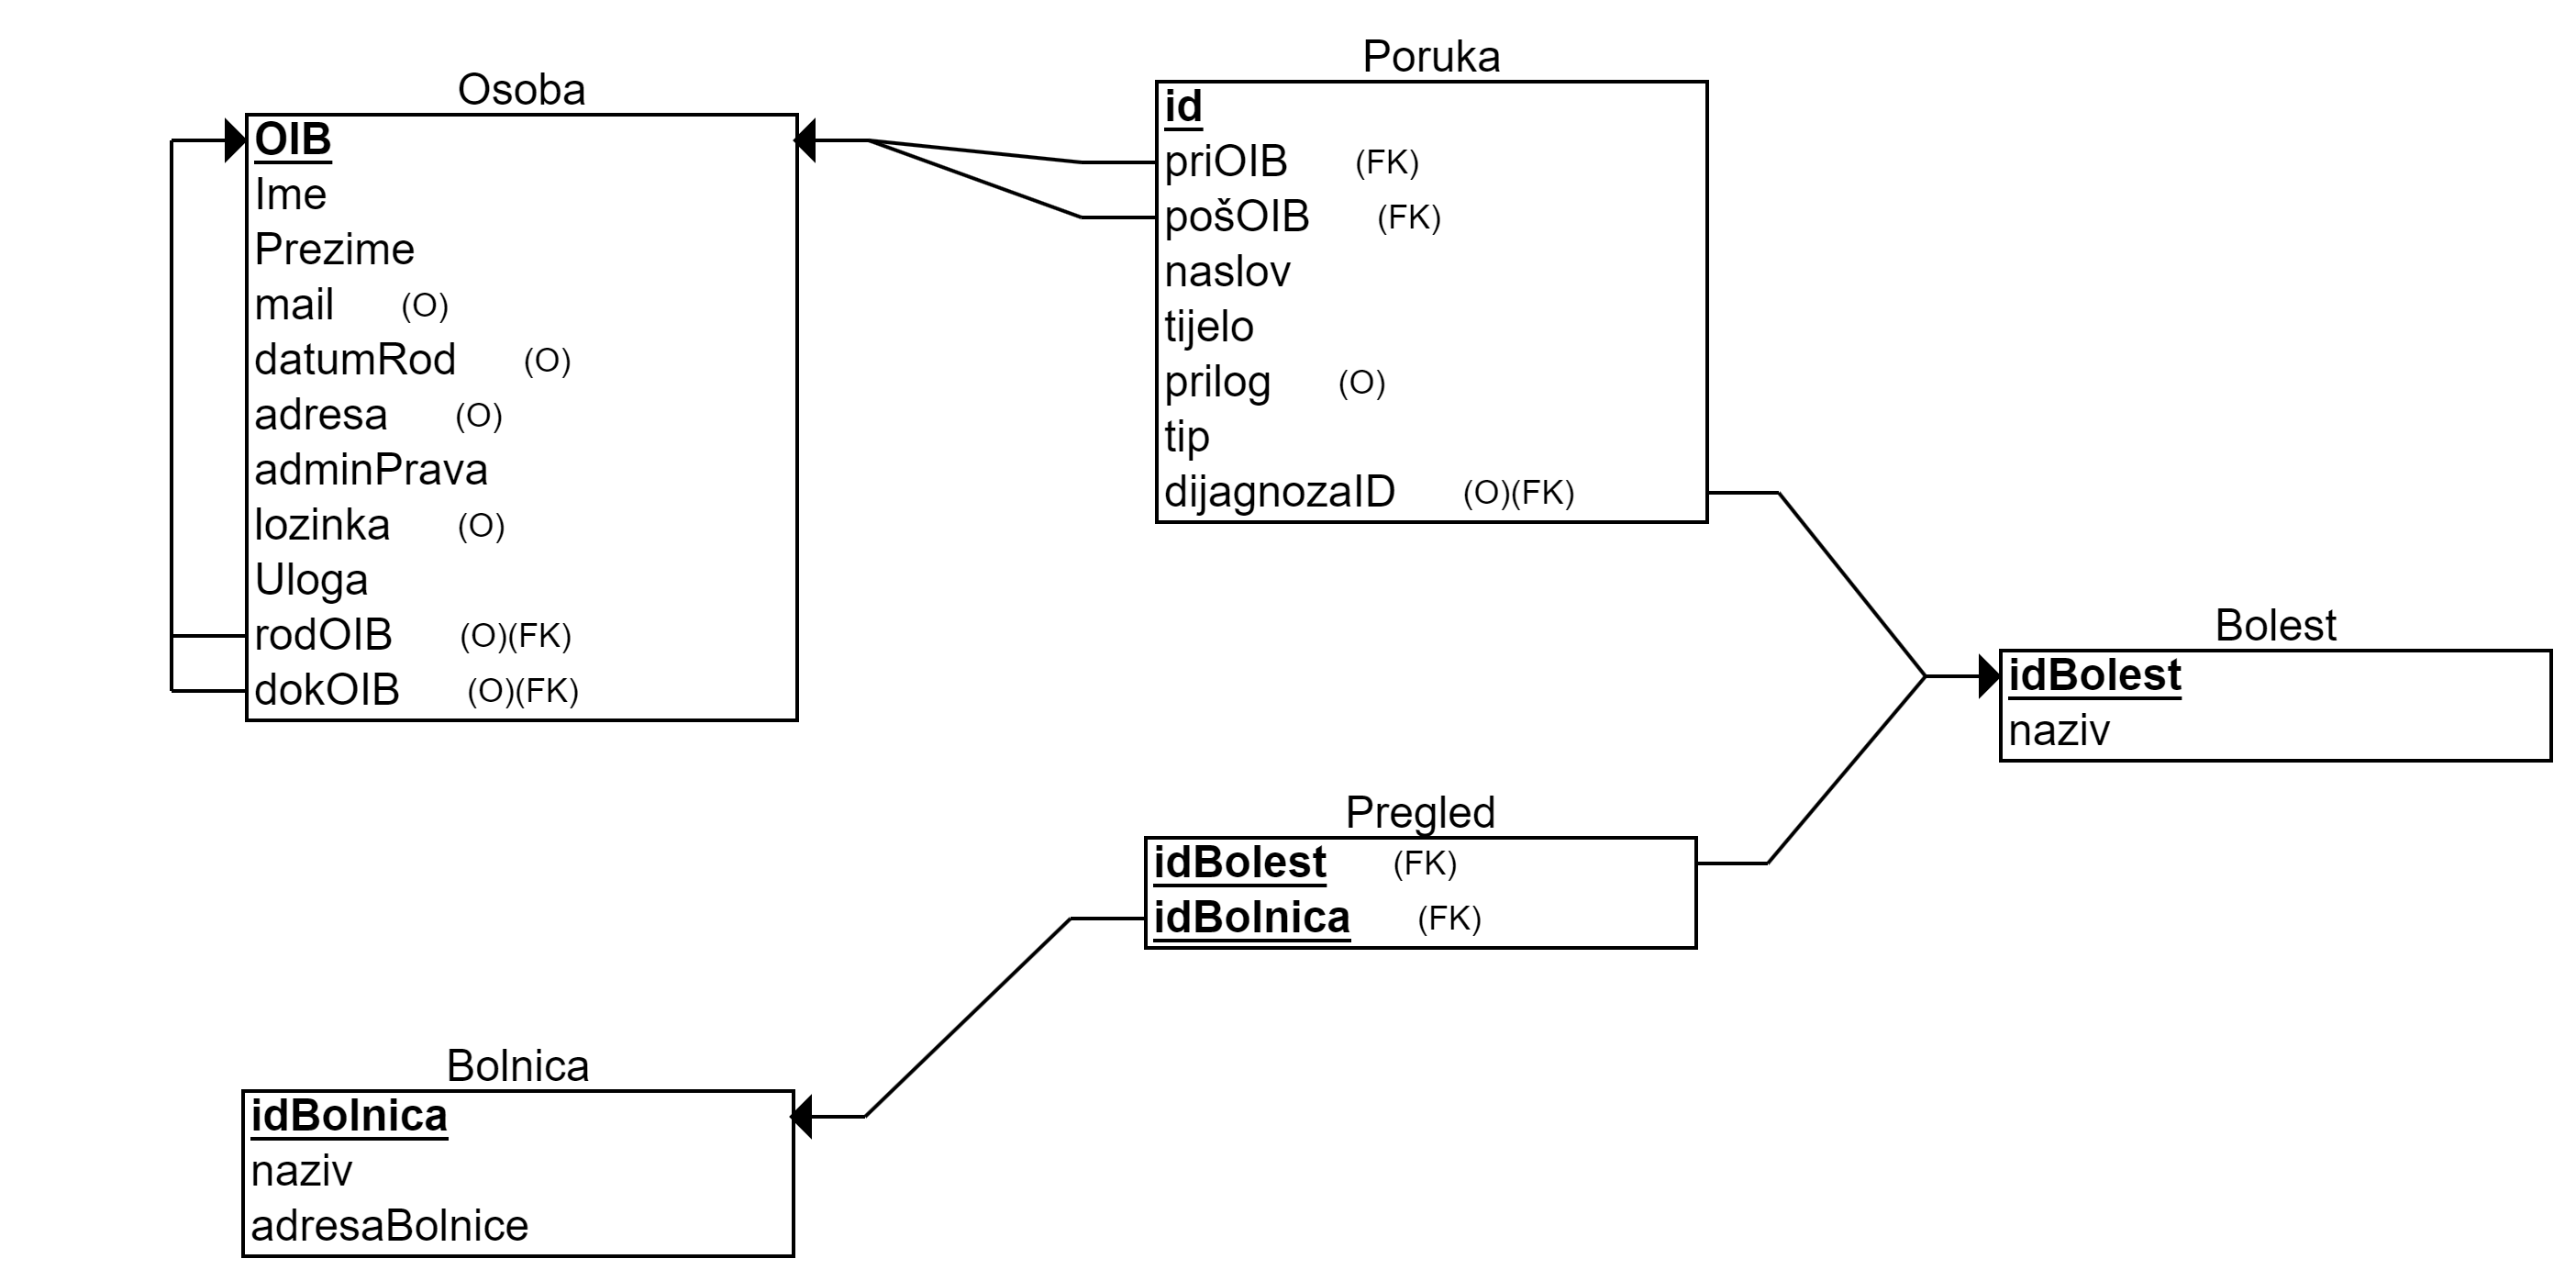
\includegraphics[width=\textwidth]{slike/dijagramBazeHigh.png} %veličina u odnosu na širinu linije
					\caption{Dijagram baze podataka}
					\label{fig:promjene10} %label mora biti drugaciji za svaku sliku
				\end{figure}
			
			\eject
			
			
		\section{Dijagram razreda}
		
			\begin{figure}[H]
				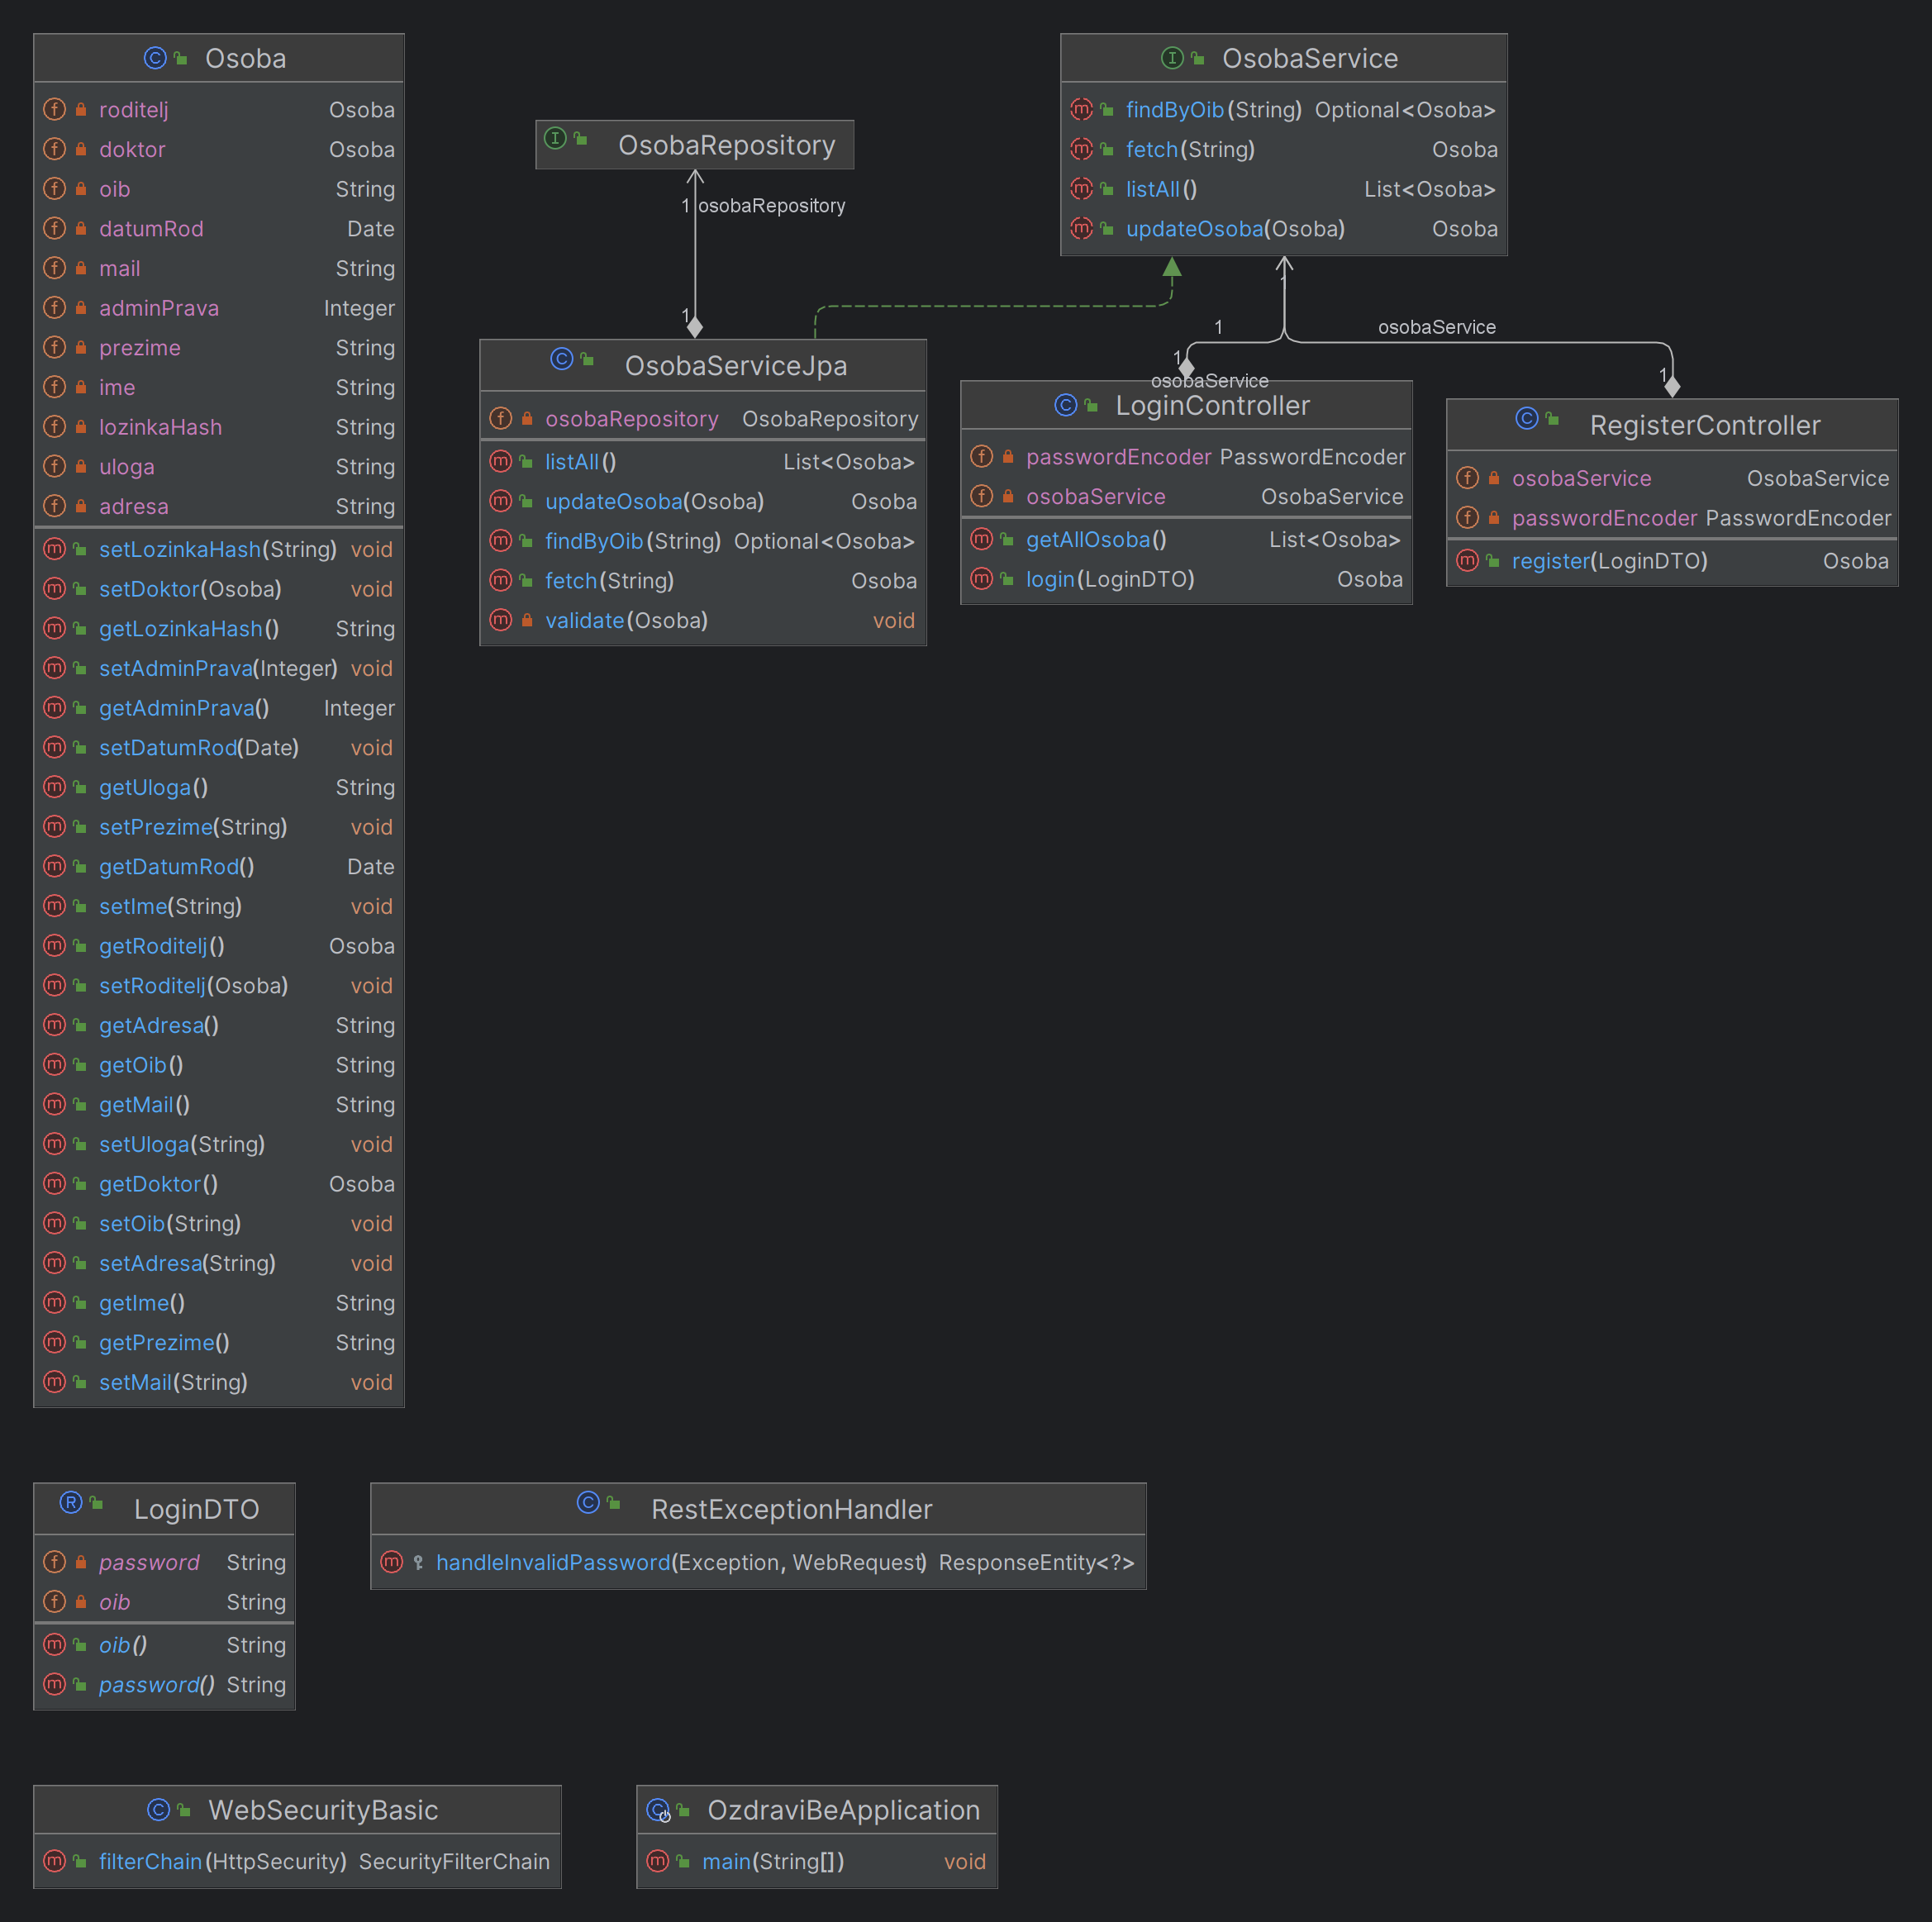
\includegraphics[width=\textwidth]{dijagrami/classDiagram1.png} %veličina u odnosu na širinu linije
				\caption{Dijagram razreda}
				\label{fig:promjene10} %label mora biti drugaciji za svaku sliku
			\end{figure}
			\

			\textit{Razred }\textbf{Osoba}
			 predstavlja entitet Osoba baze podataka. 
			Sadrži sve njegove atribute odgovarajućih tipova s pripadnim integritetskim ograničenjima, kao i gettere i settere za sve njih kako bi im Springov ORM mogao pristupiti.

			\textit{Sučelje }\textbf{OsobaRepository}
			 daje sučelje za pristup entitetu Osoba u bazi podataka preko JPA.

			\textit{Sučelje }\textbf{OsobaService}
			 opisuje operacije kojima se pristupa entitetu Osoba, 
			ne oslanjajući se na konkretnu implementaciju (tj. na Repository),
			što je u skladu sa objektnom paradigmom i omogućuje primjenu dependency injectiona.
			
			\textit{Razred }\textbf{OsobaServiceJpa}
			 predstavlja konkretnu implementaciju sučelja OsobaService koja entitetu Osoba
			pristupa preko repozitorija (tipa OsobaRepository) na kojeg pamti referencu.

			\textit{Razred }\textbf{LoginController}
			 služi za obradu zahtjeva za prijavu (login).
			Pamti referencu na apstraktni OsobaService kako bi mogao raditi operacije nad bazom Osoba.
			Također mora imati referencu na objekt tipa PasswordEncoder čiji je zadatak primijeniti hash algoritam
			na dobivenu lozinku kako bi se mogla usporediti sa hashem koji je spremljen u bazi. Članske funkcije 
			ove klase izvršavaju se prilikom primanja HTTP zahtjeva, što vrijedi općenito za Controller klase
			(tj. njihove objekte) u Springu. Članska funkcija login će na POST zahtjev s odgovarajućim podatcima
			obaviti prijavu korisnika. Članska funkcija getAllOsoba postoji isključivo za svrhe testiranja i ona će na GET zahtjev vratiti popis svih osoba
			u JSON formatu. 

			\textit{Razred }\textbf{RegisterController}
			 služi za obradu zahtjeva za registraciju (register).
			Isto kao i razred LoginController, drži referencu na OsobaService radi pristupa bazi i na PasswordEncoder
			kako bi dobivene lozinke mogao hashirati prije spremanja u bazu. Članska funkcija register će na POST
			zahtjev s odgovarajućim podatcima pokušati izvršiti registraciju novog korisnika. 

			\textit{Zapis }\textbf{LoginDTO}
			 je pomoćni Data Transfer Object zapis, koji, kao što mu ime nalaže, služi za pakiranje
			dobivenih podataka pri prijavi ili registraciji u Java objekt. 

			\textit{Razred }\textbf{RestExceptionHandler}
			 služi za hvatanje iznimki koje mogu biti bačene prilikom obrade HTTP zahtjeva u Controllerima i ovisno o iznimki
			vraća pravilan HTTP odgovor (npr. odgovor ne smije biti 500 ako se dogodi iznimka pri obradi zahtjeva jer je korisnika
			unio nepravilne podatke). Članska funkcija handleInvalidPassword će uhvatiti iznimke uzrokovane
			pogrešnim podatcima za prijavu ili registraciju i vratiti HTTP odgovor sa smislenom porukom.

			\textit{Razred }\textbf{WebSecurityBasic}
			 služi za konfiguriranje sigurnosnih postavki. U ovom trenutku su one najosnovnije.

			\textit{Razred }\textbf{OzdraviBeApplication}
			 je automatski generiran od strane Springa i sadrži ulaznu točku za izvršavanje programa.

			\

			\textbf{\textit{dio 2. revizije}}\\			
			
			\textit{Prilikom druge predaje projekta dijagram razreda i opisi moraju odgovarati stvarnom stanju implementacije}
			
			
			
			\eject
		
		\section{Dijagram stanja}
			
			
			\textbf{\textit{dio 2. revizije}}\\
			
			\textit{Potrebno je priložiti dijagram stanja i opisati ga. Dovoljan je jedan dijagram stanja koji prikazuje \textbf{značajan dio funkcionalnosti} sustava. Na primjer, stanja korisničkog sučelja i tijek korištenja neke ključne funkcionalnosti jesu značajan dio sustava, a registracija i prijava nisu. }
			
			Dijagram stanja opisuje dinamičko ponašanje dijela sustava. Na slici \ref{fig:dijagramstanja} prikazan je dijagram stanja za prijavljenog roditelja. Roditelju se nakon prijave prikazuje popis profila kojima može pristupati (profil roditelja i profili njegove djece). Odabirom pojedinog profila aplikacija roditelju prikaže poruke tog profila. Klikom na gumb za prikaz osobnih podataka profila, aplikacija roditelju pokaže iste te roditelj ima daljnju opciju promjene podataka. Ako roditelj na stranici s prikazanim porukama profila odabere pojedinu poruku, otvori se novi prozor u kojem se prikazuje poruka te karta ako se radi o obavijesti za naručeni pregled. Roditelj može na svaku poruku odgovoriti te mu se tada otvori novi prozor za sastavljanje poruke u kojem je automatski postavljen i primatelj poruke. Roditelju se prozor za sastavljanje poruke otvara i ako na stranici gdje su prikazane poruke tog profila klikne na gumb za učitavanje nalaza. Roditelj se u svakom trenutku može odjaviti ili vratiti na stranicu s popisom dostupnih profila.
			
			\begin{figure}[H]
				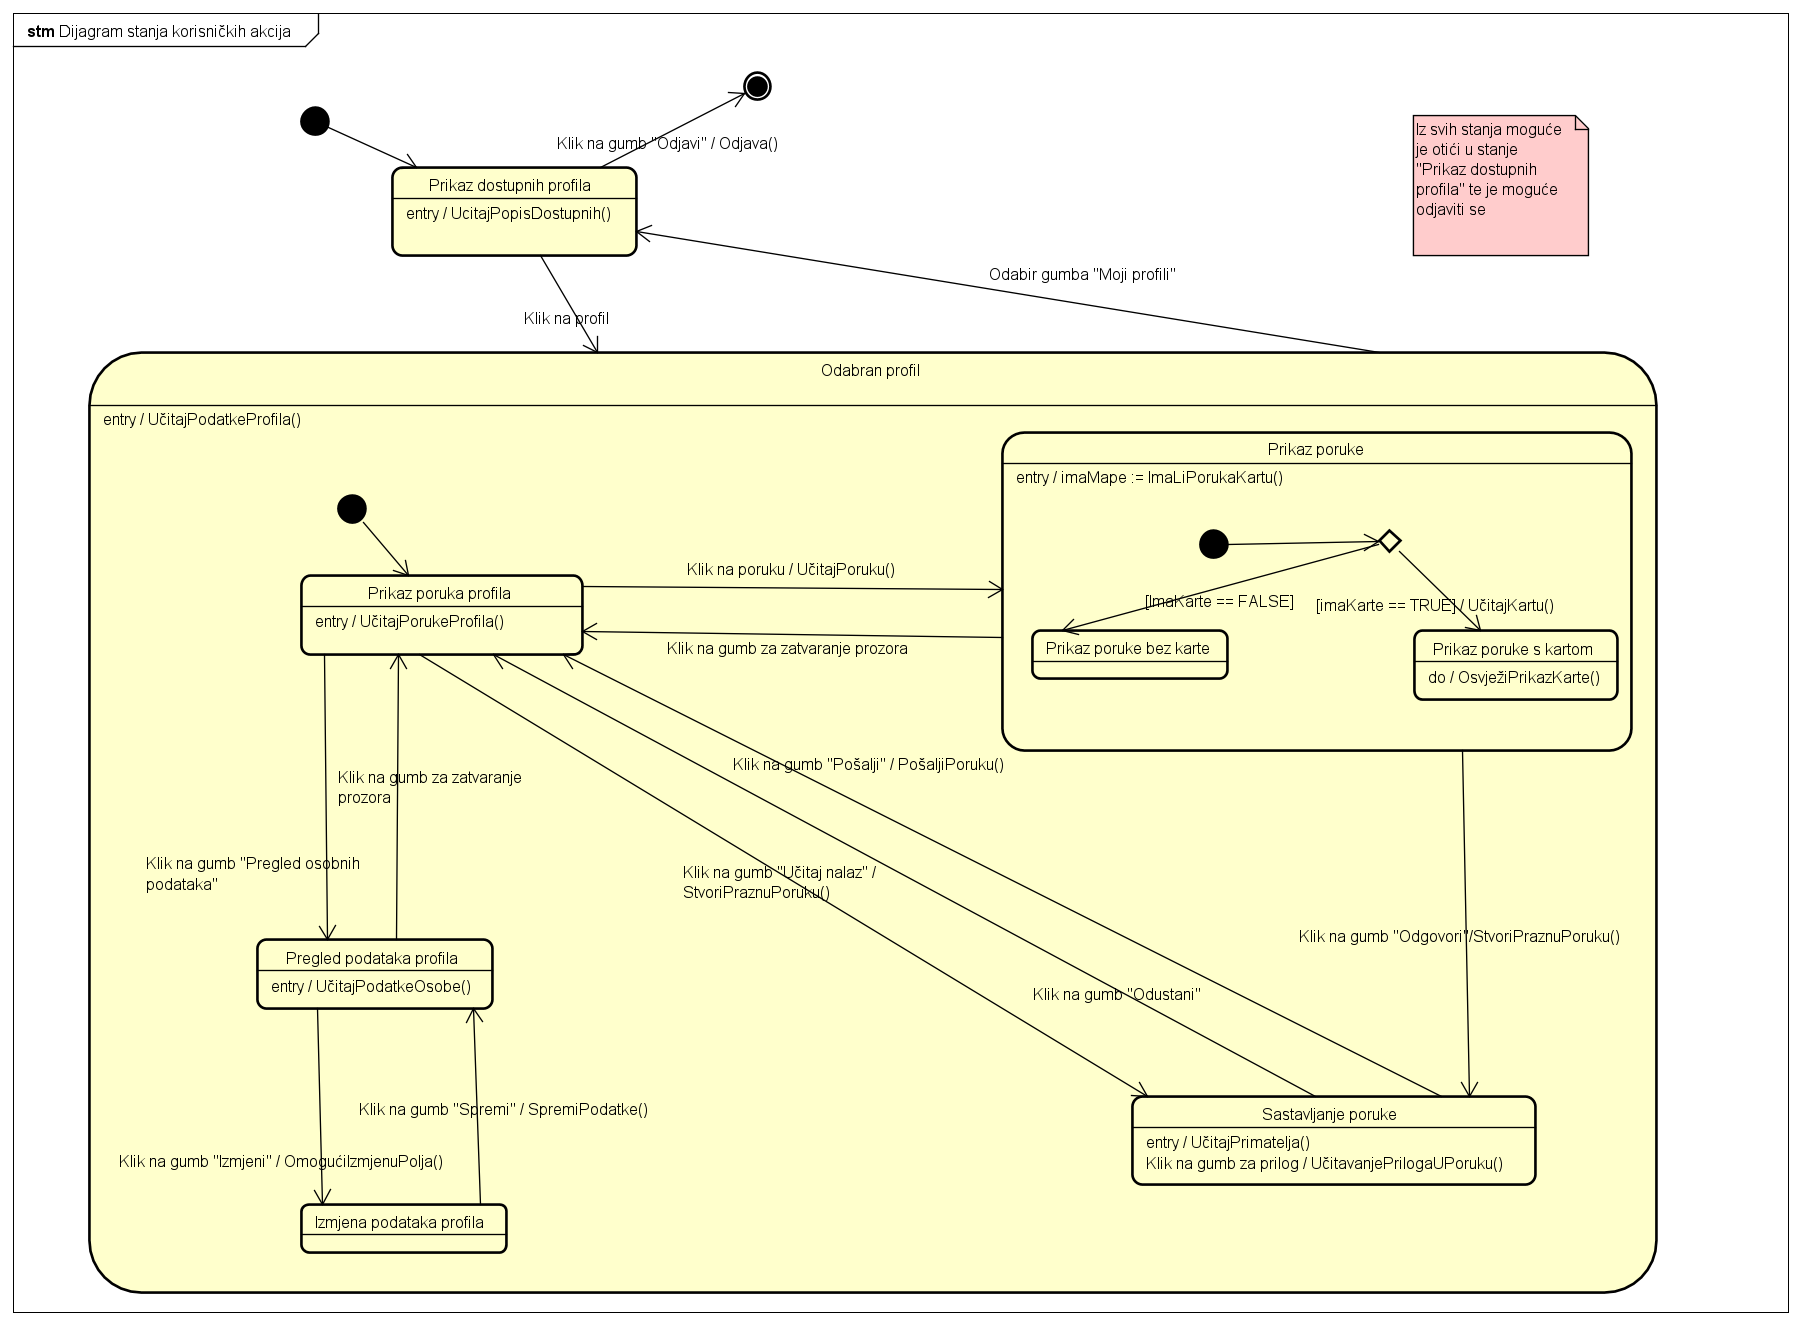
\includegraphics[width=\textwidth]{dijagrami/Dijagram stanja.PNG} %veličina u odnosu na širinu linije
				\caption{Dijagram stanja}
				\label{fig:dijagramstanja} %label mora biti drugaciji za svaku sliku
			\end{figure}
			
			
			\eject 
		
		\section{Dijagram aktivnosti}
			
			\textbf{\textit{dio 2. revizije}}\\
			
			 \textit{Potrebno je priložiti dijagram aktivnosti s pripadajućim opisom. Dijagram aktivnosti treba prikazivati značajan dio sustava.}
			 
			 Dijagram aktivnosti primjenjuje se za modeliranje upravljačkog i podatkovnog toka. Na slici \ref{fig:dijagramaktivnosti} prikazan je dijagram aktivnosti za upisivanje podataka o obavljenom pregledu kod pedijatra. Nakon što pedijatar upiše podatke za prijavu u sustav, web aplikacija iz baze podataka izvlači potrebne informacije za provjeru ispravnosti podataka. Ako su podaci neispravni, prikazuje se poruka greške, a ako su ispravni web aplikacija prijavljenom pedijatru prikaže popis djece prijavljene kod njega. Pedijatar potom bira dijete za kojeg želi upisati pregled (preduvjet za to je da je dijete prijavljeno kod njega). Nakon odabira djeteta web aplikacija pedijatru prikaže poruke s profilom tog djeteta. Pedijatar sad može odabrati opciju za unos pregleda nakon čega se otvara novi prozor u kojem pedijatar može unijeti potrebne podatke. Kada je gotov s unosom podataka, pedijatar bira opciju za slanje dijagnoze. Web aplikacija novostvorenu poruku koja sadrži podatke o pregledu pohranjuje u bazu, a pedijatru se opet prikažu poruke s profilom djeteta.
			 
			 \begin{figure}[H]
			 	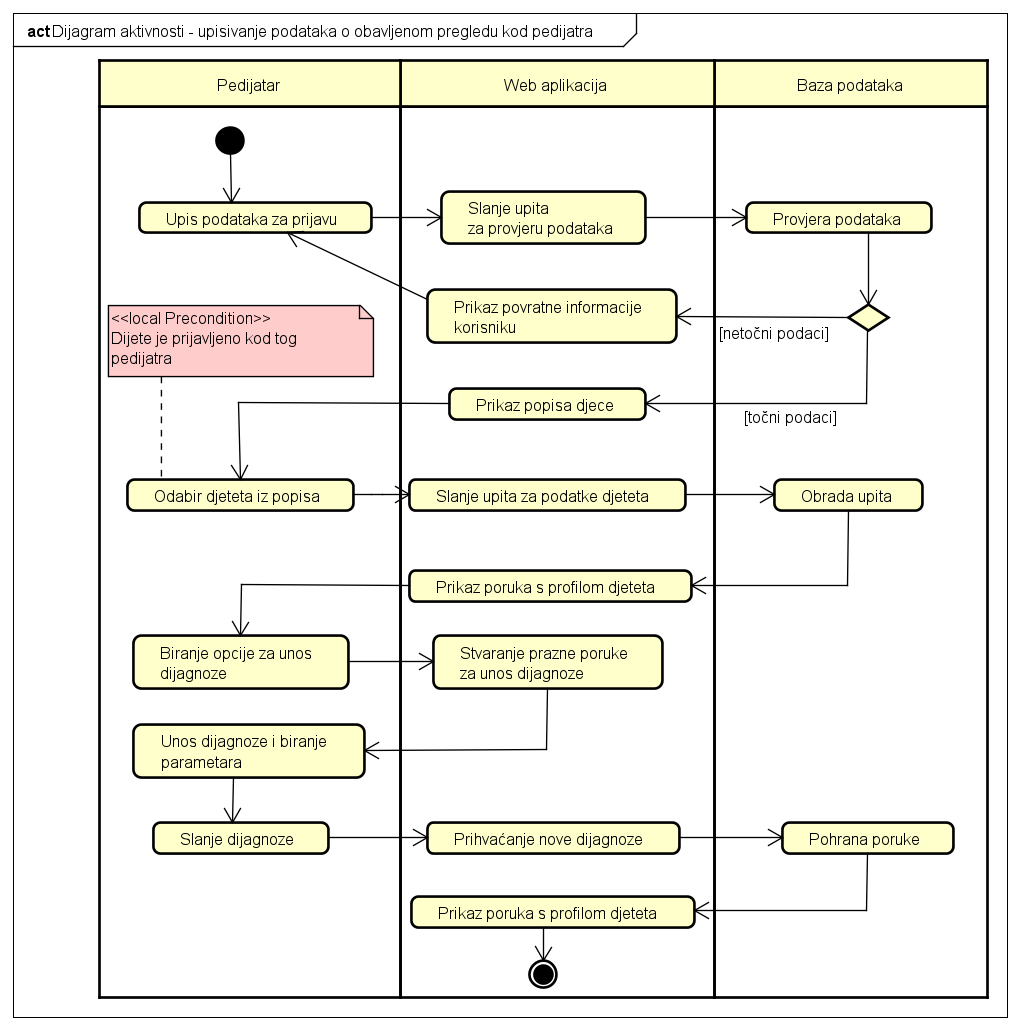
\includegraphics[width=\textwidth]{dijagrami/Dijagram aktivnosti.PNG} %veličina u odnosu na širinu linije
			 	\caption{Dijagram aktivnosti}
			 	\label{fig:dijagramaktivnosti} %label mora biti drugaciji za svaku sliku
			 \end{figure}
			
			\eject
		\section{Dijagram komponenti}
		
			\textbf{\textit{dio 2. revizije}}\\
		
			 \textit{Potrebno je priložiti dijagram komponenti s pripadajućim opisom. Dijagram komponenti treba prikazivati strukturu cijele aplikacije.}